\documentclass{beamer}

\usepackage{epstopdf}
\usepackage{float}
\usepackage{multicol}
\usepackage{chngpage}

\usetheme{Data61}

\title{Modelling and Solving the Multi-Skill Project Scheduling Problem}
\author{Kenneth Young}
% \institute, \subtitle are not implemented yet

\begin{document}

\maketitle
% alternatively use \frame[plain]{\titlepage}
% \frame{\tableofcontents}

\section{Introduction}
\subsection{Problem Definition}
\begin{frame}{Intro: The Problem}
	\pause What is the Multi-Skill Project Scheduling Problem (MSPSP)?\pause
	\begin{itemize}
		\item Activites\pause
		\item Workers\pause
		\item Skills\pause
	\end{itemize}
	\vspace{4mm}
	\alert{Aim:} Find the fastest way to complete all the activities\pause\\
	\vspace{4mm}
	Constraints\pause
	\begin{itemize}
		\item Activity constraint: Precedence relations between activities\pause
		\item Skill constraint: Activities require skills\pause
		\item Worker constraint: Workers each have a variety of skills
	\end{itemize}
\end{frame}

\subsection{Example}
\begin{frame}{Intro: Example}
	\scriptsize
	\begin{multicols}{2}
		\begin{table}
			\caption{Workers' Skills}
			\vspace{-3mm}
			\begin{tabular}{c|cccc}
				\hline
				 & Alice & Bob & Carl & Dora \\
				\hline
				{\tiny {\bf Programmer}} & - & \checkmark & \checkmark & \checkmark \\
				{\tiny {\bf DB Designer}} & \checkmark & - & - & - \\
				{\tiny {\bf Webmaster}} & \checkmark & \checkmark & - & \checkmark \\
				\hline
			\end{tabular}
		\end{table}\pause
		\begin{figure}[H]
			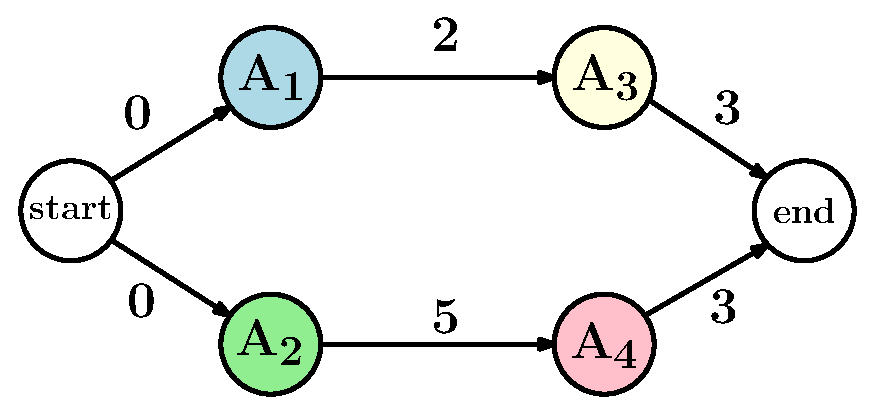
\includegraphics[width=\linewidth]{images/precgraph.eps}
			\caption{Precedence Graph}
		\end{figure}\pause
		\columnbreak

		\begin{table}
			\caption{Skill Requirement}
			\begin{tabular}{c|cccc}
				\hline
				 & $A_1$ & $A_2$ & $A_3$ & $A_4$ \\
				\hline
				{\tiny {\bf Programmer}} & - & 1 & 2 & 1 \\
				{\tiny {\bf DB Designer}} & 1 & - & - & 1 \\
				{\tiny {\bf Webmaster}} & 1 & 1 & - & - \\
				\hline
			\end{tabular}
		\end{table}\pause
		\vspace{-8mm}
		\begin{figure}[H]
			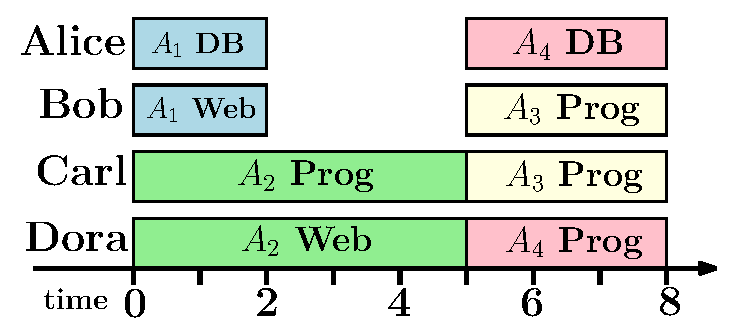
\includegraphics[width=\linewidth]{images/sched.eps}
			\caption{Schedule}
		\end{figure}

	\end{multicols}
\end{frame}

\subsection{Constraint Programming}
\begin{frame}{Intro: Constraint Programming}
	\begin{multicols}{2}
		Domain propagation
		\begin{itemize}
			\item Variables have domains of possible values
			\item Constraints reduce the size of these domains
		\end{itemize}\pause
		\columnbreak
		Nogood learning
		\begin{itemize}
			\item Learn from failures
			\item Record these failures as constraints
			\item Use these constraints to make inferences
		\end{itemize}
	\end{multicols}
\end{frame}

\subsection{Previous Work}
\begin{frame}{Intro: The Literature}
	\begin{itemize}
		\item Portuguese research group
		\begin{itemize}
			\item Principal researchers: Almeida, Saldanha-da-Gama, Correia
			\vspace{1mm}
			\item Constructive heuristics
			\vspace{1mm}
			\item Randomised search heuristics\pause
		\end{itemize}
		\vspace{2mm}
		\item French research group
		\begin{itemize}
			\item Principal researchers: Belleguez-Morineau, N\'{e}ron, Montoya
			\vspace{1mm}
			\item Exact branch and bound methods
			\vspace{1mm}
			\item Lower bounds\pause
		\end{itemize}	
		\vspace{2mm}
		\item Polish research group
		\begin{itemize}
			\item Principal researchers: Myzskowski, Skowronski
			\vspace{1mm}
			\item Randomised search heuristics
		\end{itemize}
	\end{itemize}
\end{frame}


%~~~~~~~~~~~~~~~~~~~~~~~~~~~~~~~~~~~~~~~~~~~~~~~~~~~~~~~~~~~~~~~~~~~~~~~~~~~~~~~~~%
% MODEL
\section{Model}
\subsection{Overview}
\begin{frame}{Model: Overview}
	\begin{itemize}
		\item \pause Objective\pause
		\begin{itemize}
			\item Minimise the total project duration\pause
		\end{itemize}
	\end{itemize}
	\vspace{5mm}
	\begin{itemize}
		\item Two main decisions\pause
		\vspace{2mm}
		\begin{enumerate}
			\item Scheduling decisions
			\begin{itemize}
				\item Activity start times\pause
			\end{itemize}
			\vspace{2mm}
			\item Assignment decisions
			\begin{itemize}
				\item Workers to activities
				\vspace{1mm}
				\item Skill contribution of workers
			\end{itemize}
		\end{enumerate}
	\end{itemize}
\end{frame}

\subsection{Constraints}
\begin{frame}{Model: Constraints}
	\begin{itemize}
		\item \pause Precedence relations are respected\pause
		\vspace{2mm}
		\item Workers perform only one activity at a time\pause
		\vspace{2mm}
		\item Workers cannot multi-task\pause
		\vspace{2mm}
		\item Skill requirement is satisfied
		\begin{itemize}
			\item A worker for each skill must be present to perform the activity\pause
		\end{itemize}
		\vspace{2mm}
		\item Redundant constraints
	\end{itemize}
\end{frame}

\begin{frame}{Model: Choice of Constraints}
	Unary Resource Constraint
	\vspace{1mm}
	\begin{itemize}
		\item Each worker only performs one activity at a time\pause
	\end{itemize}
	\vspace{5mm}
	Three equivalent ways of modelling\pause
	\vspace{1mm}
	\begin{enumerate}
		\item Boolean satisfiability constraint using extra decision variable\pause
		\vspace{1mm}
		\item Disjunctive global constraint\pause
		\vspace{1mm}
		\item Cumulative global constraint
	\end{enumerate}
\end{frame}


%~~~~~~~~~~~~~~~~~~~~~~~~~~~~~~~~~~~~~~~~~~~~~~~~~~~~~~~~~~~~~~~~~~~~~~~~~~~~~~~~~%
% DATA
\section{Data}
\begin{frame}{Data: Overview}
	\begin{itemize}
		\pause
		\item Generated our own data
		\begin{itemize}
			\item equivalent to the Portuguese group's data\pause
		\end{itemize}
		\vspace{2mm}
		\item Small dataset: 216 unique instances
		\begin{itemize}
			\item 20 activities
			\vspace{1mm}
			\item 10-30 workers\pause
			\vspace{1mm}
			\item \alert{13 unsolved}\pause
		\end{itemize}
		\vspace{2mm}
		\item Large dataset: 216 unique instances
		\begin{itemize}
			\item 40 activities
			\vspace{1mm}
			\item 20-60 workers\pause
			\vspace{1mm}
			\item \alert{211 unsolved}
		\end{itemize}
	\end{itemize}
\end{frame}

\begin{frame}{Data: Complexity Measures}
	\begin{enumerate}
		\item Skill Factor
		\vspace{1mm}
		\begin{itemize}
			\item varied over 4 values\pause
		\end{itemize}
		\vspace{2mm}
		\item Network Complexity
		\vspace{1mm}
		\begin{itemize}
			\item varied over 3 values\pause
		\end{itemize}
		\vspace{2mm}
		\item Modified Resource Strength
		\vspace{1mm}
		\begin{itemize}
			\item varied over 3 values
		\end{itemize}
	\end{enumerate}
	% \vspace{3mm}
	% Therefore, 36 types of instances 
\end{frame}


%~~~~~~~~~~~~~~~~~~~~~~~~~~~~~~~~~~~~~~~~~~~~~~~~~~~~~~~~~~~~~~~~~~~~~~~~~~~~~~~~~%
% EXPERIMENTS
\section{Experiments}
\subsection{Choosing Parameters}
\begin{frame}{Experiments: Constraint Choice}
	Sample of 72 small instances\pause
	\begin{figure}[H]
		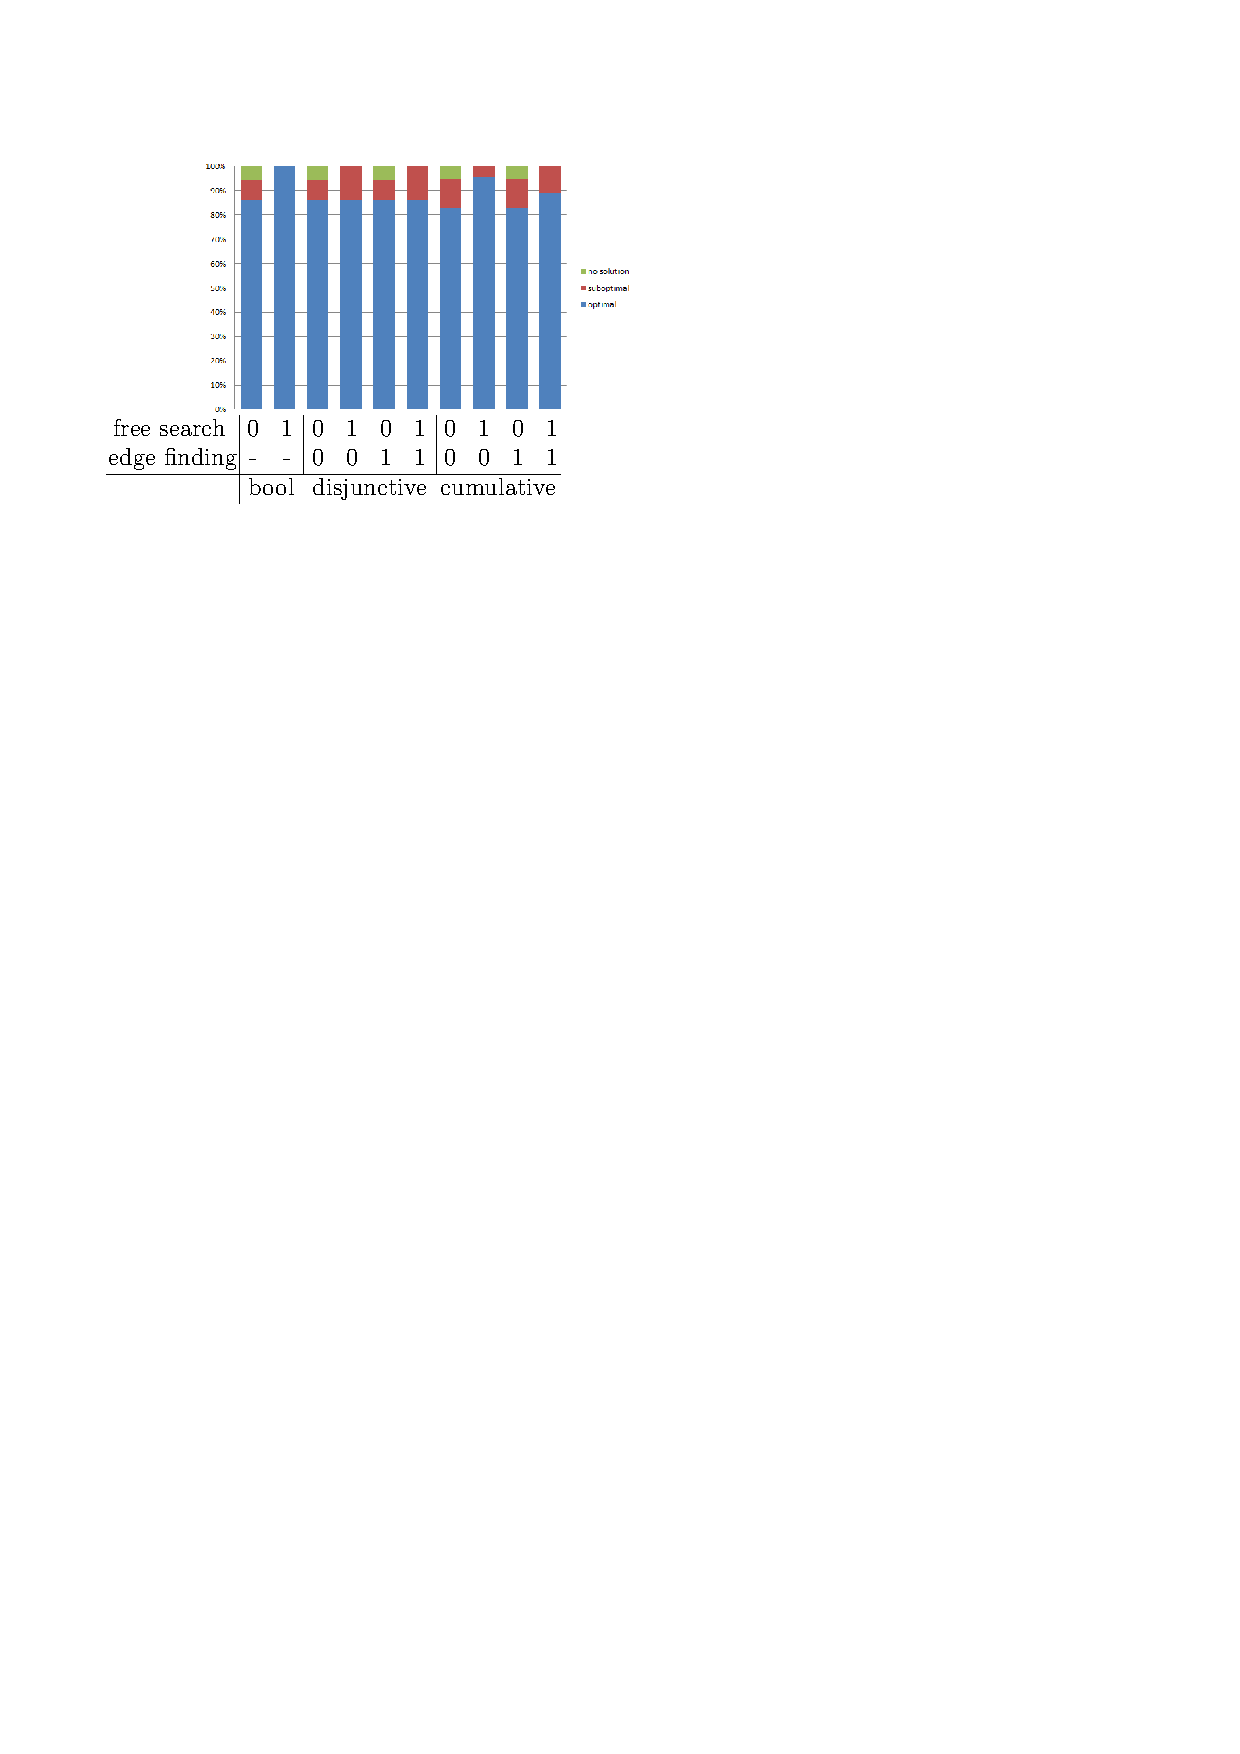
\includegraphics[width=0.8\linewidth]{images/constChoice.pdf}
	\end{figure}
\end{frame}

\subsection{Results}
\begin{frame}{Experiments: Search Strategies}
	\begin{itemize}
		\item \pause Start time variables
		\vspace{2mm}
		\item \pause Start time variables, then contrbution of each worker
		\vspace{2mm}
		\item \pause Activity-based
	\end{itemize}
\end{frame}

\begin{frame}{Experiments: Results}
	\begin{itemize}
		\item Tested on all 216 small instances
		\item Time limit of 5 minutes \pause
	\end{itemize}
	\begin{table}[H]
		\begin{adjustwidth}{-.9in}{-.9in}
		\centering
		\scriptsize
		\begin{tabular}{r|rrrrrr}
			\hline
			search strategy & \#no soln & \#sub-opt & \%gap & \#optimal & \%optimal & avg. runtime  \\
			\hline
			default & 0 & 0 & 0.00 & 216 & 100.00 & 3.25s \\
			start &  0 & 1 & 2.50 & 215 & 99.54 & 1.26s \\
			start then worker & 0 & 0 & 0.00 & 216 & 100.00 & 2.89s \\
			\bf{start then skill} & \bf{0} & \bf{0} & \bf{0.00} & \bf{216} & \bf{100.00} & \bf{1.63s} \\
			activity-based & 0 & 1 & 2.50 & 215 & 99.54 & 0.82s\\\hline
		\end{tabular}
		\end{adjustwidth}
	\end{table}
\end{frame}

%~~~~~~~~~~~~~~~~~~~~~~~~~~~~~~~~~~~~~~~~~~~~~~~~~~~~~~~~~~~~~~~~~~~~~~~~~~~~~~~~~%
% CONCLUSION
\section{Conclusion}
\subsection{Summary}
\begin{frame}{Summary}
	\begin{itemize}
		\item Applied the constraint programming solver chuffed to the MSPSP\pause
		\vspace{2mm}
		\item Generated a set of benchmark instances\pause
		\vspace{2mm}
		\item Found an effective model formulation\pause
		\vspace{2mm}
		\item Solved all small instances
	\end{itemize}
\end{frame}

\subsection{Future Work}
\begin{frame}{Future Work}
	\begin{itemize}
		\item Apply activity-based search to the large dataset\pause
		\vspace{2mm}
		\item Create a more structured search procedure in the chuffed
	\end{itemize}
\end{frame}

\begin{frame}{Acknowledgements}
	\begin{itemize}
		\item Dr. Andreas Schutt
		\vspace{2mm}
		\item Dr. Thibaut Feydy
		\vspace{2mm}
		\item Adrian Goldwaser
	\end{itemize}
\end{frame}

\begin{frame}{}
	\centering
	{\Large Thanks for listening!\vspace{1cm}\\
	Questions?}
\end{frame}

\end{document}
